\documentclass[a4paper,11pt,exos]{nsi} % COMPILE WITH DRAFT
\usepackage{hyperref}

\pagestyle{empty}
\begin{document}


\classe{\terminale Comp}
\titre{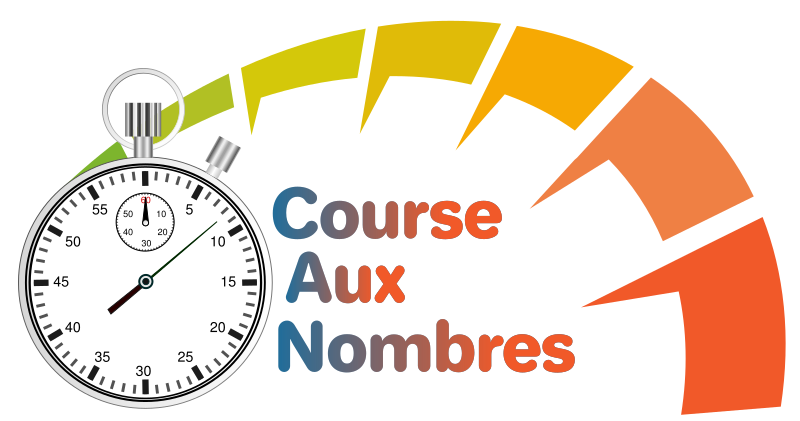
\includegraphics[width=3cm]{CAN.png} Entrainement 1}
\maketitle

\begin{enumerate}[itemsep=1em]
	\item $7 \times 0{,}8=$  $\ldots$
	\item $7+\dfrac{3}{7}= $ $\ldots$
	\item Développer et réduire l'expression $(2x-1)(3x+2)$.
	\item Donner l'écriture décimale de :  $4+5\times 10^{-3}+7\times10^2$.
	\item Résoudre l'équation $10x-10=0$.
	\item $4$ croissants coûtent  $4{,}40$ €.  Combien coûtent $2$ croissants ?
                        
	\item Calculer la fréquence de boules noires parmi ces boules :\\
          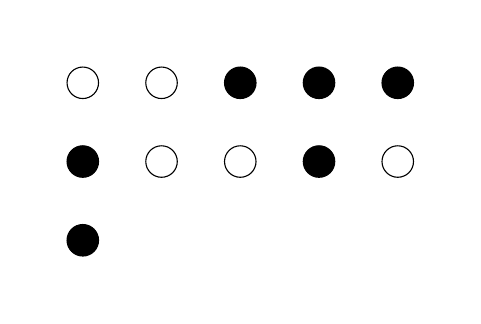
\begin{tikzpicture}[baseline]

    \tikzset{
      point/.style={
        thick,
        draw,
        cross out,
        inner sep=0pt,
        minimum width=5pt,
        minimum height=5pt,
      },
    }
    \clip (-0.7,-2.7) rectangle (4.7,0.7);
    	
	 \filldraw[color={black},fill={white}] (0,0) circle (0.2);
	
	 \filldraw[color={black},fill={white}] (1,0) circle (0.2);
	
	 \filldraw[color={black},fill={black}] (2,0) circle (0.2);
	
	 \filldraw[color={black},fill={black}] (3,0) circle (0.2);
	
	 \filldraw[color={black},fill={black}] (4,0) circle (0.2);
	
	 \filldraw[color={black},fill={black}] (0,-1) circle (0.2);
	
	 \filldraw[color={black},fill={white}] (1,-1) circle (0.2);
	
	 \filldraw[color={black},fill={white}] (2,-1) circle (0.2);
	
	 \filldraw[color={black},fill={black}] (3,-1) circle (0.2);
	
	 \filldraw[color={black},fill={white}] (4,-1) circle (0.2);
	
	 \filldraw[color={black},fill={black}] (0,-2) circle (0.2);

\end{tikzpicture}\\
	\item Calculer l'expression  $x^2+3x-10$ pour $x=-1$.
	\item Calculer la moyenne de :
            $7\,\,\,; \,\,\,9\,\,\,; \,\,\,3\,\,\,; \,\,\,1$.
	\item $30$ $\%$ de $40= $ $\ldots$
	%\item  $9{,}1$ m$^3=$ $\ldots$ L
\end{enumerate}


\vspace*{1cm}
Mon temps : $\ldots$\\[.5em]
Mon score : $\ldots$/10

\newpage
\titre{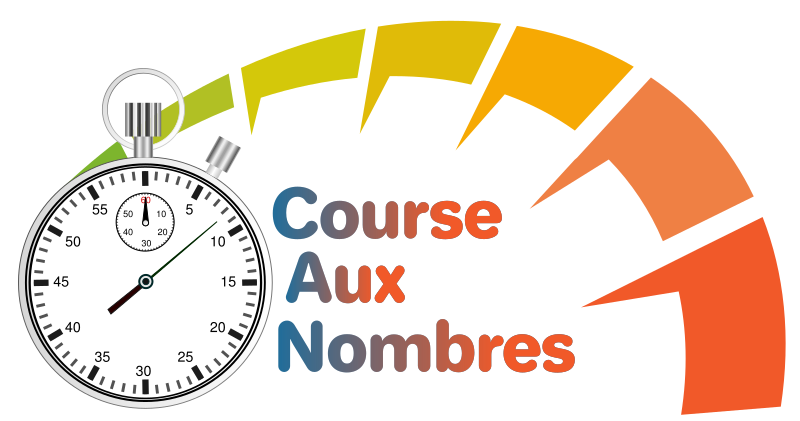
\includegraphics[width=3cm]{CAN.png} Corrigé de l'entrainement 1}
\maketitle

\textcolor{UGLiBlue}{
\begin{enumerate}[itemsep=1em]
    \item $7 \times 0{,}8=7\times 8\times 0,1=5{,}6$
    \item $7+\dfrac{3}{7}= \dfrac{49}{7}+\dfrac{3}{7}=\dfrac{52}{7}$
    \item \begin{tabbing}
        $(2x-1)(3x+2)$\=$=2x\times 3x+2\times 2x-1\times 3x-1\times 2$\\
        \>$=6x^2+4x-3x-2$\\
        \>$=6x^2+x-2$
    \end{tabbing}
    \item $4+5\times 10^{-3}+7\times10^2=4+0{,}005+700=704{,}005$
    \item On se ramène à une équation du type $a\times x=b$ :\\
              $\begin{aligned}
              10x-10&=0\\
             10x&=10\\
                                  x&=\dfrac{10}{10}=\dfrac{1{\color[HTML]{2563a5}\boldsymbol{\times10}} }{1{\color[HTML]{2563a5}\boldsymbol{\times10}}}=1
             \end{aligned}$\\
              L'équation $10x-10=0$ a pour solution $x=1$.
    \item $4$ croissants coûtent  $4{,}40$ €, donc
                           $2$ croissants coûtent $2$ fois moins, soit : \\
                           $4{,}40\div 2=2{,}20$ €.
    \item La fréquence est donnée par le quotient : $\dfrac{\text{Nombre de boules noires}}{\text{Nombre total de boules}}=\dfrac{6}{11}$.
    \item 
                Pour $x=-1$, on obtient : $x^2+3x-10=(-1)^2+3\times (-1)-10=-12$.
    \item La moyenne est donnée par : $\dfrac{7+9+3+1}{4}=\dfrac{20}{4}=5$.
    \item           Prendre $30$ $\%$  de $40$ revient à prendre $3\times 10$ $\%$  de $40$.\\
                Comme $10$ $\%$  de $40$ vaut $4$ (pour prendre $10$ $\%$  d'une quantité, on la divise par $10$), alors
                $30$ $\%$ de $40=3\times 4=12$.
    %\item Comme $1$ m$^3$= $1000$ L, $9{,}1$ m$^3=9\,100$ L.
\end{enumerate}}
\end{document}